\section{ Question 2  }\label{sec:q2} 

\textit{Consider a body that moves in an low-eccentric elliptic orbit around the sun. You may assume that the body is only subject to the gravitational attraction of the sun, described by gravitation potential, and the radiation pressure of the sunlight. The equations of motion of this body are:}
\begin{equation}\label{eq:2_1}
\begin{split}
    \ddot{r}-r\dot{\theta} ^{2}=-\dfrac {\mu }{r^{2}}+\dfrac {F}{m}\sin \left( \delta \right) \\
    \dfrac {d}{dt}\left( r^{2}\dot{\theta} \right) =\dfrac {F}{m}r\cos \left( \delta \right) \\
\end{split}
\end{equation}
where:
\begin{equation} \label{eq:2_2}
    F = C_R \frac{W S}{c}
\end{equation}

If one assumes that the sunlight is radiated in a radially symmetrical way, and that the orbiting body is spherical, then the acceleration of the body because of radiation pressure can be formulated as:
\begin{equation}\label{eq:2_3}
    \dfrac {F}{m}=\dfrac {3}{4}\dfrac {C_{R}W_{s}R^{2}_{s}}{c \rho R}\dfrac {1}{r^{2}}
\end{equation}
for a given body follows that:
\begin{equation}
    \frac{F}{m} = \frac{\alpha}{r^2}
\end{equation}
where $\alpha$ is a constant. 

\subsection{2a}
\textit{Indicate what the parameters in equations \ref{eq:2_1}, \ref{eq:2_2}, and \ref{eq:2_3} mean.}\\
Parameters:
\begin{itemize}
    \item $\ddot{r}$ is the radial acceleration of the body in orbit
    \item $r$ is the radial distance of the body in orbit w.r.t. the CoM of the sun
    \item $\dot{\theta}$ is the angular velocity of the body in orbit w.r.t. the sun
    \item $\mu$ is the gravitational parameters of the sun (assuming $m_{sun} \gg m_{body}$)
    \item $F$ is the force due to the solar radiation pressure action on the body in orbit
    \item $m$ is the mass of the body in orbit
    \item $\delta$ is the angle of F w.r.t. the tangential velocity of the body in orbit (see figure \ref{fig:delta})
\end{itemize}

\begin{figure}[H]
    \centering
    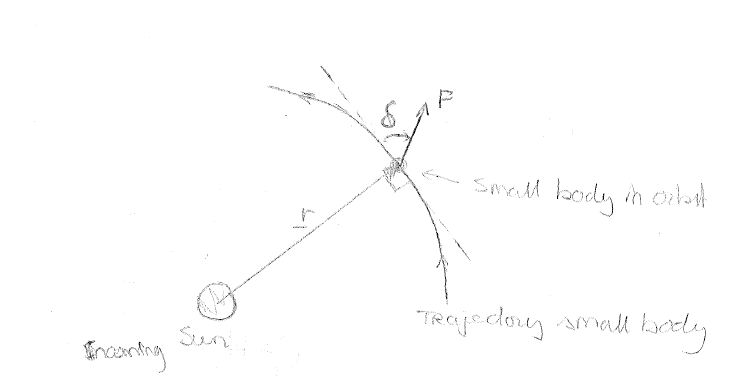
\includegraphics[width=0.4\columnwidth]{Figures/2a.png}
    \caption{Definition of angle $\delta$}
    \label{fig:delta}
\end{figure}

Furthermore:
\begin{itemize}
    \item $C_R$ is the reflectivity coefficient of the body in orbit
    \item $W$ is the power density of the incoming beam
    \item $W_S$ is the power density of the sun
    \item $S$ is the illuminated surface area of the body in orbit 
    \item $c$ is the speed of light
    \item $R_S$ is the radius of the sun
    \item $\rho$ is the density of the body in orbit
    \item $R$ is the radius of the spherical body in orbit
    \item $\alpha$ is a constant defined as $\frac{3 C_R W_S R_S^2}{4 c \rho R}$
\end{itemize}

Finally, what the terms mean:
\begin{itemize}
    \item $\ddot{r}$ is the acceleration of the body in orbit
    \item $(-r \dot{\theta})$ is the centrifugal acceleration on the body in orbit, caused by the rotation of the sun
    \item $\frac{\mu}{r^2}$ is the gravitational acceleration of the sun
    \item $F/m \cdot sin(\delta) \, and \, F/m \cdot cos(\delta)$ are accelerations due to the solar radiation pressure
    \item $r^2 \dot{\theta}$ is the angular momentum of the body in orbit
    \item $\frac{d}{dt} (r^2 \dot{\theta})$ is the change of angular momentum over time.
\end{itemize}

\subsection{2b}
\textit{Explain why generally for the computation of the effects of solar radiation pressure on the orbit of the body, a doppler-term and an abberation-term must be taken into account. These phenomena can be described by:} 
\begin{equation}
    W'=W\left( 1-\dfrac {\dot{r}}{c}\right) \quad ; \quad \gamma =\dfrac {r \dot{\theta} }{c}
\end{equation}
\\
The energy of a photon can be represented by 
\begin{equation}
    E_{ph} = h \cdot f
\end{equation}
where h is the Planck constant and f the frequency of the photon.
Since it was assumed that the sun emits energy in a radially symmetric manner, if the body is in a circular orbit, the frequency of the body will be unchanged.
If the radius of the body in orbit increases (because of increasing $\ddot{r}$) the frequency of the energy will decrease compared to if the body was in a circular orbit. Therefore, the incoming power density will decrease.
If the radius of the body in orbit decreases due to decreasing $\ddot{r}$, the frequency of the incoming energy will increase w.r.t. the body in a circular orbit and therefore the power density will increase.
These two effects are the doppler-effect and can be described by $W'=W\left( 1-\dfrac {\dot{r}}{c}\right)$.

The aberration effect is the phenomenon that the incoming beam of the sun falls under a small angle onto the body in orbit, due to the travel time of the incoming beam. The explanation of this phenomenon is more clearly indicated with the following sketches:
At $t_0$, the sunlight leaves the surface of the sun and travels towards the body in orbit.
\begin{figure}[H]
    \centering
    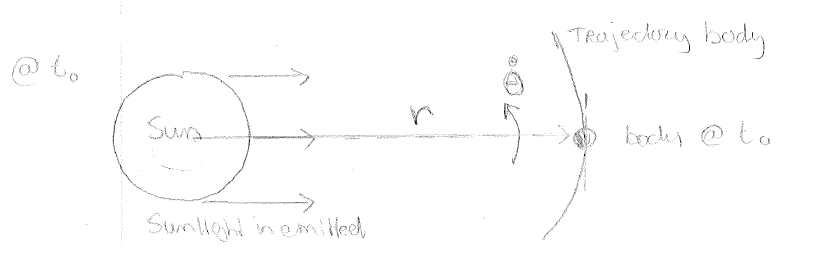
\includegraphics[width=0.5\columnwidth]{Figures/2b.png}
    \caption{Situation at $t_0$}
    \label{fig:aberration1}
\end{figure}

Then, at $t_0 + \Delta t$, this sunlight reaches the body in orbit, under an angle $\gamma$.
\begin{figure}[H]
    \centering
    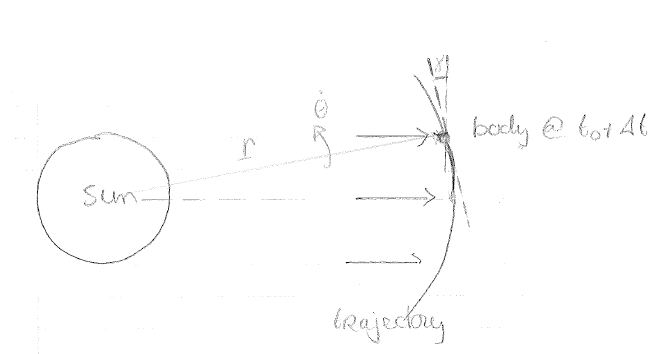
\includegraphics[width=0.5\columnwidth]{Figures/2b2.png}
    \caption{Situation at $t_0 + \Delta t$}
    \label{fig:aberration2}
\end{figure}

This incoming angle can be described by:
\begin{equation}
    \gamma = \frac{r \cdot \dot{\theta}}{c}
\end{equation}


\subsection{2c}
\textit{Derive how with the effects of question 2b, a first-order approximation of equations \ref{eq:2_1} can be written as:}
\begin{equation}
\begin{split}
    \ddot{r}-r\dot{\theta} ^{2} = -\dfrac {\mu -\alpha }{r^{2}}-\dfrac {\alpha \dot{r}}{cr^{2}} \\
     \dfrac {d}{dt}\left( r^{2}\dot{\theta} \right) = -\frac{\alpha \dot{\theta}}{c}
\end{split}
\end{equation}
\textit{Using these equations, provide a description of the two effects of the radiation pressure on the motion of the orbiting body (Poynting-Robertson effect).} \\

Filling in the doppler-term into the given relation for $F/m$:
\begin{equation}
    \dfrac {F}{m}=\dfrac {3}{4}\dfrac {C_{R}\cdot W'_{s}\cdot R_{S}}{C\cdot \rho\cdot R}\cdot \dfrac {1}{r^{2}} = \dfrac {3}{4}\dfrac {C_{R}\cdot W_s \cdot R_{S}}{C\cdot \rho \cdot R} \left[ 1-\dfrac {\dot{r}}{c}\right]  \cdot \dfrac {1}{r^{2}}
\end{equation}
and so:
\begin{equation}
    \dfrac {F}{m}=\dfrac {\alpha }{r^{2}}\left[ 1-\dfrac {\dot{r}}{c}\right] 
\end{equation}

For the aberration effect, the angle $\delta$ is increased by angle $\gamma$. If we assume that the effect of $\delta \approx 90^{/circ}$:
\begin{equation}
\begin{split}
    \sin \left( \delta +\gamma \right) \approx \sin \left( \dfrac {\pi }{2}+\gamma \right) = \cos ( \gamma ) \\
    \cos \left( \delta +\gamma \right) \approx \cos \left( \dfrac {\pi }{2}+\gamma \right) = - \sin ( \gamma ) \\
\end{split}
\end{equation}
If we further assume that the aberration angle $\gamma$ is small, we get:
\begin{equation}
\begin{split}
    \sin ( \gamma ) \approx \gamma \quad and so \quad \sin(\delta) \approx 1 \\
    \cos ( \gamma ) \approx 1 \quad and so \quad \cos(\delta) \approx -\gamma \\
\end{split}
\end{equation}

If we apply the previous to the equations of motion: 
\begin{equation}
\begin{split}
    \ddot {r}-r\cdot \dot{\theta} ^{2}=-\dfrac {\mu }{r^{2}}+\dfrac {\alpha }{r^{2}}\left[ 1-\dfrac {\dot{r}}{c}\right] \cdot 1 = -\dfrac {\left( \mu -\alpha \right) }{r^{2}}-\dfrac {\alpha \cdot \dot{r}}{c\cdot r^{2}} \\
    \dfrac {d}{dt}\left( r^{2}\cdot \dot{theta} \right) =\dfrac {\alpha }{r^{2}}\left[ 1-\dfrac {\dot{r}}{c}\right] \cdot -\gamma  = -\dfrac {\alpha \cdot \dot{\theta} }{c}+\dfrac {\dot{r}\cdot r\cdot \dot{\theta} \cdot x}{r\cdot c^{2}} \approx -\dfrac {\alpha \cdot \dot{\theta} }{c}
\end{split}
\end{equation}

The Poynting-Robertson effect describes the tendency of the solar radiation pressure to reduce the acceleration due to the gravitational attraction of the sun. It causes a drag-like force that reduces the acceleration in the radial direction and in the tangential (circumferential) direction.  


\subsection{2d}
\textit{As $\alpha$ increases, the effects of radiation pressure on the orbit of the body will increase. Which kinds of bodies will have a large value of $\alpha$?} \\
If we look at the definition of $\alpha$:
\begin{equation}
    \alpha = \frac{3 C_R W_S R_S^2}{4 c \rho R}
\end{equation}
we see that $\alpha$ increases if a body is more reflective ($C_R$), less dense ($\rho$) or has smaller radius ($R$). The speed of light, and the power density and radius of the sun do not depend on the body in orbit.



\subsection{2e}
\textit{It can be shown that generally $\alpha = \mu$ for a value between $R=0.09 /, - /, 7 \, \mu m$. In reality, the sun radiates 97\% of its energy with wavelengths between $0.3 /, - /, 0.9 \, \mu m$. What can be said about particles in our solar system whose size is comparable to these wavelengths, and about the fact that we see the sun as a "bright disc", rather than a "blurry light source"?} \\

If a particle has the dimension of order of the wavelength, $\alpha = \mu$. Looking at the first equation of motion, in this case the gravitational attraction is counteracted, so there will only be a 'drag-like' term, which will accelerate the body away from the sun.
Since these particles are accelerated away from the sun, the sun can be seen as a clear disk, since the particles are "blown away".